% !TeX root = ../main.tex

\chapter{相关技术简介}
本章简要介绍与本文密切相关的几种技术及框架,整个系统基于这几种技术
进行开发。在本章,我们将对ESL建模、Simpy仿真框架
以及一些相关技术进行详尽的阐述。

\section{ESL建模介绍}
ESL(Electronic System Level)设计和验证是一种电子设计方法。基本方法是
使用高级语言或使用图形化工具对整个系统的行为进行建模。新的语言不断出现,
现在常用SystemC来完成作为一种抽象的建模语言。

ESL是许多世界领先的片上系统设计公司的既定方法,并且越来越多地用
于系统设计。ESL最初是作为一种“没有实现链接”的算法建模方法,现在正
在演变成一套互补的方法,使嵌入式系统设计、验证和调试成为可能,一直到定
制SoC的硬件和软件实现\cite{41}。

ESL设计在更高级的抽象层次上描述SoC系统,设计师可以使用ESL设计方法构建适合自己的
ESL开发环境。ESL搭建起了软件和硬件之间重要的桥梁。在电子系统及建模中,首先在顶层
建立较高抽象级的硬件虚拟模型,包括处理器、总线、存储器以及其他外设模型。然后将应用
程序映射到所建立的系统级的抽象模型,执行仿真分析和评估,给出功能执行结果和性能评估报告
,从而对系统级的功能性能给出正确的设计,ESL设计流程图\cite{42}如图2.1所示。

\begin{figure}
  \centering
  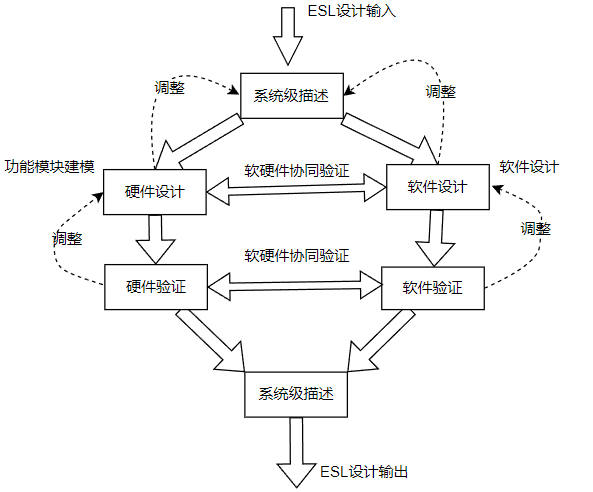
\includegraphics[width=0.7\textwidth]{ESL设计流程图.png}
  \caption{ESL设计流程图}
  \label{fig:badge}
\end{figure}

\section{SimPy仿真框架介绍}
SimPy是一个基于标准Python的基于过程的离散事件仿真框架。它的事件
调度器基于Python的生成器,也可用于异步网络或实现多代理系统(具有
模拟和真实通信)。

SimPy中的进程是由Python中的生成器函数定义。所有进程都存在于一个
环境中。它们通过事件与环境以及彼此交互。在它们的生命周期中,它们会创建
事件并创建yield以等待它们被触发。当一个进程产生一个事件时,该进程被挂起。
SimPy 在事件发生时恢复进程(我们说事件被触发)。多个进程可以等待同一个事件。
SimPy 以它们产生该事件的相同顺序恢复它们。同时,SimPy中一个重要的事件类型
为Timeout,这种类型的事件在经过一定量的(模拟)时间后触发。它们允许进程在
给定时间内休眠(或保持其状态)。所有事件都可以调用Environment进程所在的的
适当方法来创建。

SimPy 提供了三种类型的容器,可用于同步进程或对拥塞点进行建模。第一种为resource,
支持优先级和抢占的共享资源;第二种为container,用于在过程之间共享同质物质的资源,
无论是连续的还是离散的;第三种为store,用于存储支持特定对象请求的可能无限数量的对
象的共享资源。此外,我们还可以自定义资源类型的实现。

  \section{多目标优化介绍}
  在我们的对架构进行设计空间探索的过程中,目标值通常都不止一个,在多目标优化问题中各个目标之间也
  许会有冲突,无法同时取得最优。以遗传算法为代表的许多进化算法\cite{20},具有生成多个点并进行多方向搜索的
  特征,因此非常适合求解这种最优解的搜索空间非常复杂的多目标优化问题\cite{21}。


  多目标优化问题是在给定约束条件的前提下,求多个目标函数的最大或最小的问题\cite{22}。在多个目标函数中,有
  的可能是最小化目标函数,有的可能是最大化目标函数。多个目标之间可能会拥有不同的单位,也可能在优
  化某个目标时损害其他目标。但这并不意味着多目标优化问题可能没有最优解,事实上是可以有的,为了求
  出比较合理的解,这里引入多目标优化问题的合理解集——Pareto最优解\cite{23}。


  在求解单目标问题时,可以在所有候选解中选出唯一最好的解。但是在多目标优化问题里,由于各个目标之间
  可能存在冲突,所以最优解不一定只有一个。我们如下定义多目标的最优解:

  给定一个多目标优化问题minf(x),设X*属于Ω,如果不存在X属于Ω,使得满足以下条件:对于f(x)的任意子目标函数
  fi(x)都有fi(X)≤fi(X*),同时至少存在一个子目标函数fi(x)使得fi(X)< fi(X*)那么,我们称X*是一个
  强Pareto最优解\cite{24}。

  \section{SQLite数据库介绍}
  SQLite以其小巧、方便使用以及遵循ACID事务特性的优点受到开发人员的广泛喜爱,是当前使用最多的
  小型数据库之一\cite{25}。SQLite由D. Richard Hipp设计开发。在编写导弹驱逐舰上运行的设备控制程序的时候
  ,他产生了设计SQLite的想法\cite{26}。SQLite几乎支持当前所有的主流操作系统,如Android、IOS和Windows等
  ,还能在Python、Java、C\#等语言下使用,同样也支持ODBC接口。相比传统数据库如MySQL、PostgreSQL 
  等,SQLite的数据处理速度要快得多\cite{27},并且它在运行时只需要占用非常低的资源,通常仅仅需要几百K的计算机
  内存,因此它被众多嵌入式产品所采用。

  \section{仿真平台整体介绍}
  整个轻量级仿真平台由整个一起完成,为了更好的介绍设计实现
  的硬件平台相关的模块和了解仿真平台进行业务的整体流程,接下来主要介
  绍下仿真平台的整体架构、业务仿真进行的流程以及业务仿真在其他模块上的执行。

\subsection{仿真平台整体架构}
轻量级仿真平台建模整体分为硬件平台模块建模以及软件平台模块。硬件平台模块分为:Processor模块、总线互联模块
以及Memory模块;软件平台模块主要分为:输入处理模块以及调度器模块。仿真平台功能模块示意图如图2.2所示:

\begin{figure}
  \centering
  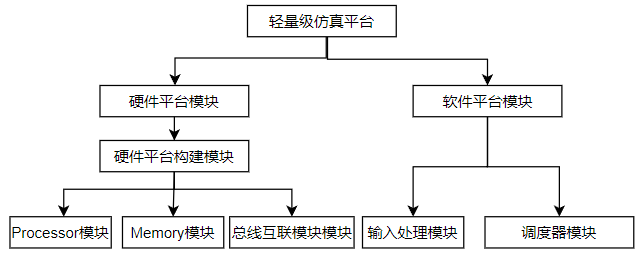
\includegraphics[width=1\textwidth]{仿真平台功能示意图.png}
  \caption{仿真平台功能模块示意图}
  \label{fig:badge}
\end{figure}

\subsection{仿真平台业务仿真流程}
仿真平台的实现是为了在芯片正式生产之前对芯片系统架构以及功能进行验证,所以需要通过
真实的用例在仿真平台上执行验证。仿真平台的业务仿真流程图如图2.3所示:

\begin{figure}
  \centering
  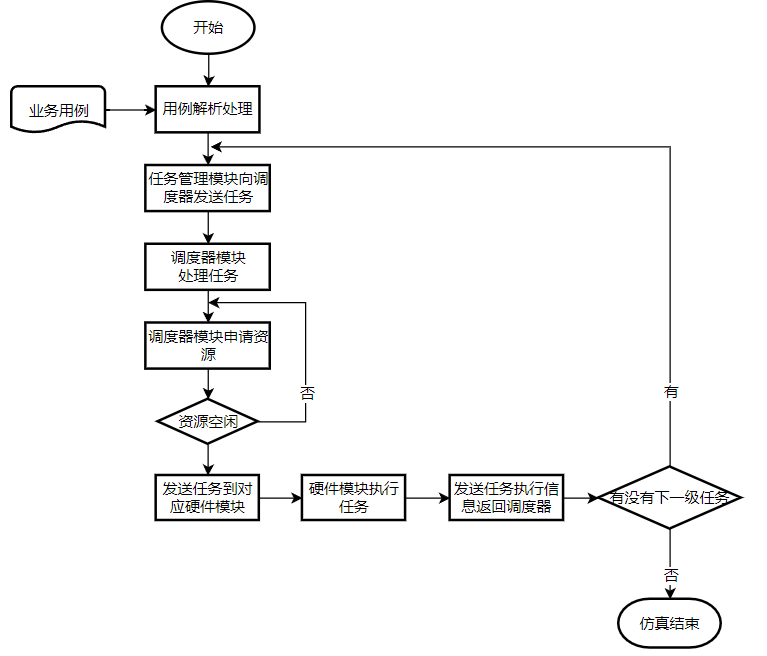
\includegraphics[width=0.9\textwidth]{仿真平台业务仿真流程图.png}
  \caption{仿真平台业务仿真流程图}
  \label{fig:badge}
\end{figure}

接下来简要的介绍整个业务仿真流程的执行,为了更好的理解本文后面设计的硬件平台模块,
下面着重介绍仿真平台与其有交互模块的设计原理以及功能。

轻量级仿真平台的输入任务模型是实例级别的数据流图模型,任务之
间以数据为触发关系,任务之间的触发为实时触发。当任务的输入数据
全部就绪后,该任务实例才会开始执行,一旦任务执行完毕,其输出数
据被触发搬运。整体的任务的数据流图示例图如图2.4所示。

\begin{figure}
    \centering
    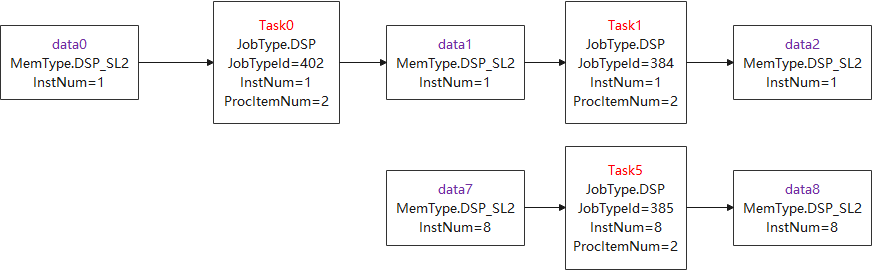
\includegraphics[width=1\textwidth]{任务数据流图示例图.png}
    \caption{任务数据流图示例图}
    \label{fig:badge}
\end{figure}

仿真平台的任务用例输入类型是描述了所有任务相关信息的
Excel文件,包括任务类型、任务执行的所属调度器、任务的
输入输出数据,数据的大小类型等等。平台初始化时通过
SaeSimulaor单实例中的load\_task\_praph方法解析任务信息
文件,并通过TaskGraphMgnt类管理。

TaskGraphMgnt类通过ExcelReader类里的方法读取输入任务用
例的Excel表,将任务信息遍历读取,根据任务用例中任务具
体信息将任务根据自身信息生成不同类型的任务对象,将数
据信息生成DataInst类对象。在Graph类中由多种类型的节
点,如图2.4任务流图示例图所示每个节点之间双向连接。
为每个TaskInst节点配置input\_data和output\_data两个字
典,为每个DataInst节点配置producer和consumer两个字典,
在Graph类中读取任务实例和数据实例,并根据在任务用例文
件中任务和数据之间关系,分别将任务实例和数据实例填入
不同节点的各自的两个字典中,并且将数据和任务之间依赖
关系作为边设为edge\_list。在读取excel的过程中构造图
的结构,并不断地将TaskInst和DataInst以及结合他们之
间的映射关系加入Graph对象中。

TaskGraphMgnt模块将所有任务全部解析并读取到Graph对象中后,当仿真系统发出
仿真执行的指令后,TaskGraphMgnt模块按照任务顺序将任务发送到调度器模块。

调度器模块负责整体任务调度,观察并接收TaskGraph Manager中就绪
任务,根据任务信息将任务分到不同子模块去分配资源,并分配到具
体硬件上去执行任务,同时接收硬件返回的response,将任务信息同
步,释放资源并触发下一级任务。调度器模块还负责管理device资源
和memory资源。调度器模块分为任务分配TOP模块、任务调度SCH模块、
资源管理RES模块几个子模块。调度模块具体结构图如图2.5所示。
  
\begin{figure}[h]
    \centering
    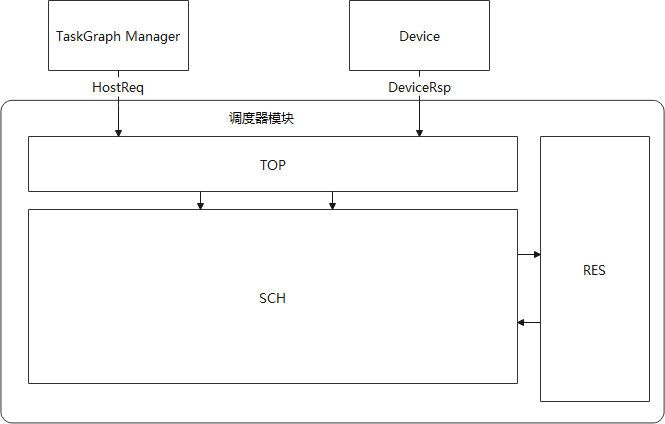
\includegraphics[width=0.8\textwidth]{调度器模块结构图.png}
    \caption{调度器模块结构图}
    \label{fig:badge}
\end{figure}
  
TOP模块负责接收任务以及硬件模型以及内部子模块发来的响应。通过
任务信息,以及响应类别,通过不同的线程将不同类别的任务分别分
到各个子模块处理。
  
SCH模块负责给任务分配资源(包括硬件模型资源CU以及硬件IP、内存
资源等等),根据任务携带的信息将任务分配给之前分配的硬件IP进
行具体的处理。
  
RES模块负责管理各个核的私有内存(包括L1D、PL2);公共内存资
源(如SL2等);管理Device资源,每个ALA支持32个Device,每个D
evice分为多个CU,CU为每个硬件模型外的任务等待队列;管理硬件
资源(如DMA、HAC等等)。其他模块通过调用这个模块的方法来申
请和释放资源。

调度器模块通过Schdule模块读取TaskGraphMgnt对象里的Graph
任务图对象读取出来。Graph对象形式是有向无环图类型,Schdule
模块先遍历有向无环图,找到DAG图中没有入度的节点即为第一个
任务或数据,将实例输入到调度器模块,由TOP模块接收判断类型,
根据信息类型转发到SCH模块。

TOP模块负责接收外部模块发送过来的任务图中实例信息以及硬件模
型处理任务完成后发送回来的响应,按照实例或者响应分开处理。
RES模块负责管理各个核的私有内存(包括L1D、PL2);公共内存
资源(如SL2等);管理Device资源。SCH模块负责向RES模块申请
管理的硬件资源和内存资源。并将任务信息或数据信息发送到申
请好的硬件IP中进行处理。

在调度器模块发送任务到具体硬件上执行后,当发生数据搬运时,
模块与模块之间的数据交互是通过总线互联模块进行的。

在仿真平台中,在不同模块之间通过总线进行通讯,而总线在不同模块上
的端口则是Port模块。针对端口设计的可扩展性,我们以Moudule Port 
Base为基础,采用Master/Slave方式。在仿真平台中,所有端口采用双
向绑定机制,即在Master端可以调用Slave端的方法.

仿真平台中现在主要有两种模块间通讯接口,一种为硬件模型模块间的接
口:Virtual Master Port和Virtual Slave Port,另一种是总线内部子
模块之间的流水线通讯接口VBusPipeLineMasterPort与VBusPipeLineSlavePort。
Port模块的关系类图如图2.6所示:
\\
\\

\begin{figure}
    \centering
    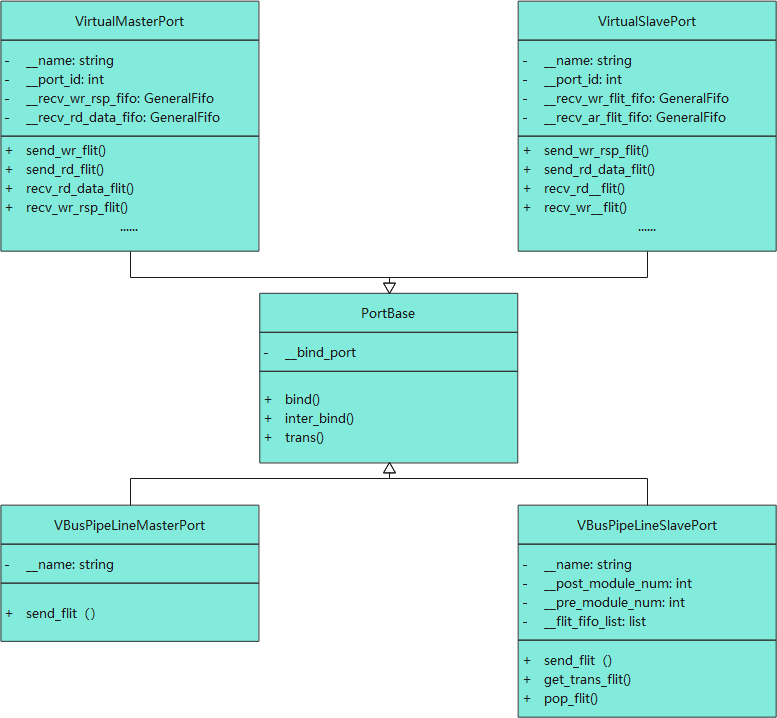
\includegraphics[width=0.8\textwidth]{Port模块关系类图.png}
    \caption{Port模块关系类图}
    \label{fig:badge}
\end{figure}

Master Device在硬件实例化的时候创建对应的VirtualMasterPort,
Slave Device在硬件实例化的时候创建对应的VirtualSlavePort。
Master Device一般是Processor模型,
硬件IP实例化时通过调用ProcessorBase的方法add\_port创建
Port端口。Slave Device一般是Memory模块。在平台构建
时,VirtualMasterPort和VirtualSlavePort通过硬件平台配
置表上的信息进行绑定。这两种端口都由PortMgnt进行管理,

在仿真平台硬件模块中,所有数据信息的传输都是通过总线模块进行,
所有的数据传输都是通过Port模块拆分封装成Flit格式的数据包经过
总线模块从一个硬件模块发送到另一个硬件模块。对应不同模块之间
总线模块是不可视的,能接触的只有Port,当Master设备发送数据到
对应Port上的操作如图MasterPortMgnt实现流程图所示。

\begin{figure}
  \centering
  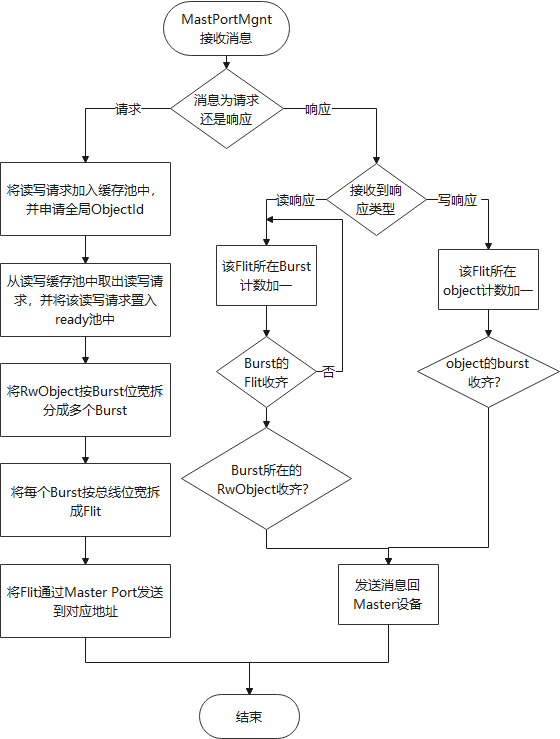
\includegraphics[width=0.7\textwidth]{MasterPortMgnt实现流程图.png}
  \caption{MasterPortMgnt实现流程图}
  \label{fig:badge}
\end{figure}

总线处理模块的主要功能是地址译码、优先级仲裁以及模拟每个
flit的传输。BUS模块中一共有四种通道,分为写通道、读地址通道、
写响应通道和读数据通道。每个通道都有一套独立的译码模块和仲裁
模块,各个模块之间通过端口连接,使用Fifo实现数据消息的传输。
\\
\\
\\

\begin{figure}
    \centering
    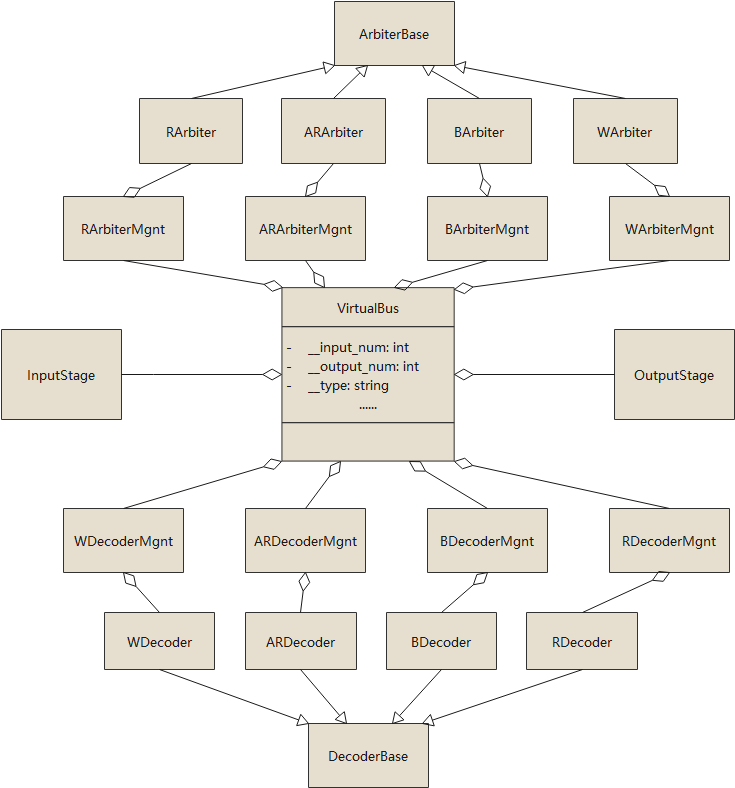
\includegraphics[width=0.7\textwidth]{BUS模块关系类图.png}
    \caption{BUS模块关系类图}
    \label{fig:badge}
\end{figure}

InputStage模块在整个BUS模块中的作用是作为外部Master Device与
内部沟通的桥梁。主要的工作流程是接收Master Device发送来的flit,
并将flit发送到对应的译码模块;以及将来自仲裁模块的flit发送回
Master Device。

OutputStage模块在整个BUS模块中是模块内部与Slave设备沟通的桥梁。
主要的工作的流程是接收来自总线模块内部发送来的flit,并将flit发
送到对应的Slave设备的Port模块;或者将Slave设备Port返回的响应发
送到对应的Decoder模块上。

BUS模块的每个通道都有独立的译码模块,但读数据通道和写响应通道的
译码模块都是对响应的译码,处理逻辑相同,我们将读数据通道和写响
应通道的译码器模块合二为一。

Arbiter模块的作用是对同一通道来自不同Decoder模块发送过来的
flit进行传输顺序的仲裁。现在仲裁模块的算法采用的轮询算法,
但在轮询算法的基础上回尽可能的保证同一个Burst的flit能够连
续发送。BUS模块的的类图如图2.8所示:

  \section{本章小结}
  本章从仿真平台建模开始介绍了ESL建模的概念,并且详细介绍了我们在实际建模过程中使用的仿真框架SimPy。
  接下来介绍了在设计空间探索中使用的遗传算法工具库Geatpy,介绍了其基本结构以及使用,同时说明了在我们
  实际设计空间探索过程中由于目标值有多个,介绍了多目标优化的基本知识以及使用遗传算法的原因。最后介绍了
  我们所使用的持久化数据的SQLite数据库。

  在了解了相关技术之后,在第三章我们将阐述该仿真平台及设计空间探索的需求分析。


  

